\documentclass{ctexart}
\begin{document}
\title{计算物理作业 11}
\author{刘畅, PB09203226}
\maketitle

{\bf [作业11]}: 模拟二维DLA的生长过程, 如对原模型作变动则更佳.

\section{算法}
二维DLA的算法是这样的: 初始时刻, 一个粒子放在 lattice 的中心, 作为初始的
cluster. 算法的每一步都在一个半径为 $r$ 的圆的随机位置释放一个粒子,
让它做随机游走, 如果碰到 cluster, 就把这个粒子加入这个 cluster.
如果跑出了半径为 $2r$ 的圆外(或整个lattice的外面), 这个粒子就作废.
算法在成功地在 cluster 中增加了给定数量的粒子后结束.

\section{程序}
这个问题中, 和前面一样, 我们用一个二维 \verb|bool| 型数组来表示
整个 lattice. \verb|true| 表示这个位置有粒子在 cluster 中,
\verb|false| 表示这个位置还没有被占用. 这个数组在堆上分配:
(\verb|main()|)
\begin{verbatim}
bool (*lattice)[CLUSTER_DIM] = (bool (*)[CLUSTER_DIM])
    malloc(CLUSTER_DIM * CLUSTER_DIM * sizeof(bool));
\end{verbatim}
然后要将这个数组初始化成 \verb|false|, 中心设成 \verb|true|
(\verb|dla_simulation()|):
\begin{verbatim}
    /* initialize the cluster */
    for (i = 0; i < dim; i++)
        for (j = 0; j < dim; j++)
            lattice[i][j] = false;
    lattice[dim/2][dim/2] = true;
\end{verbatim}

按照前面的算法, 接下来要在半径为 $r$ 的圆上随机释放一个粒子.
(\verb|dla_simulation()|):
\begin{verbatim}
  theta = rand_norm() * 2.0 * CONST_PI;
  x = dim/2 + radius * cos(theta);
  y = dim/2 + radius * sin(theta);
\end{verbatim}
再进行随机游走 (\verb|random_walk()|):
\begin{verbatim}
  do {
      i = sample_unif_dir();
      x += delta_x[i];
      y += delta_y[i];
      if (lattice[x][y]) {
          *px = x - delta_x[i];
          *py = y - delta_y[i];
          return true;
      }
  } while ( (0 <= x) && (x < dim) && (0 <= y) && (y < dim) &&
        (pow(x-dim/2,2) + pow(y-dim/2,2) < pow(max_radius,2)) );
  return false;
\end{verbatim}
上面的代码中, \verb|sample_unif_dir()| 从4个方向中随机挑选一个,
然后将相应的 $\Delta\vec r$ 增加到 $\vec r=(x,y)$ 上. 如果新的位置
被占据了, 旧的位置就被记录下来, 并且(在 \verb|dla_simulation()| 中)
把相应位置的 \verb|lattice| 设置成 \verb|true|. 否则, 就继续行走,
直到粒子离开半径为 \verb|max_radius| 的圆, 或离开整个 lattice.

这个过程被反复执行 \verb|nparticles| 次, 表明一共生长了
\verb|nparticles| 个粒子. 代码在 \verb|dla_simulation()|,
\verb|for| 循环那一行.

\section{结果}
我们将格点设成 $1024\times1024$, 行走 4096 步 (见 \verb|main()|).
将结果做成图:
\begin{center}
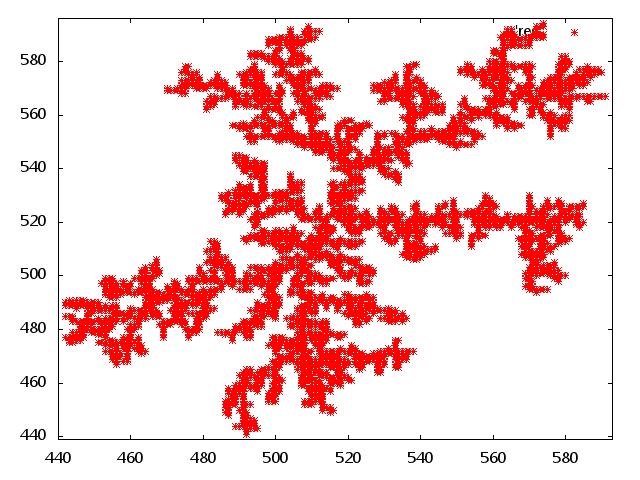
\includegraphics[width=4in]{res.png}
\end{center}
可以看到和书上的结果是一致的.

\end{document}